\hoofdstuk{Conclusion and recommendations}

At the start of this thesis the following question was asked: `How can license plate information be gathered from the images of a smartphone camera using software?'. This question was then divided into two more specific questions because it was too broad. Those questions were: `How can the software be optimized to work in a correct way from within a mobile device?' and `What are the limitations of such an application?'. Using the information gathered during the course of the project, these questions will now be answered.

\paragraaf{How can the software be optimized to work in a correct way from within a mobile device?}

Because smartphones are limited devices when it comes to processing power, when creating such an application these limitations must be taken into account. This was solved using two different approaches: multi-threading and buffers.

Starting with multi-threading, this technique allows an application to share its processing load with every processor core in the smartphone. The application uses four threads for its main four components: the UI thread, the band localization thread, the plate localization thread and the text recognition thread. This allows for, in the case of the smartphone used to test the application, a dedicated core for every thread.

The buffers approach takes into consideration that a smartphone does not have enough processing power to process images at real-time. The outputs of every thread, with the exception of the text recognition thread because its output is handled immediately, are therefore stored within a buffer so they can be processed in their own time. Each buffer has their own limitations and rules which are related to the importance of the data stored within. There are 3 different buffers: the frames buffer, the bands buffer, and the plates buffer. The frames buffer stores the video frames capture with the smartphone's camera and has a maximum size of 1 and a discard policy. This means that every time a new frame is available, if there was still a unprocessed frame within the buffer this frame will be discarded. This prevents old unprocessed frames to accumulate and therefore keep the processed data as recent as possible.


% In the case of the Frames  This allows for a lower chance of missing the capture of an image of a plate because the application was busy processing the last captured image.

\paragraaf{What are the limitations of such an application?}

\begin{figure}[ht]
    \centering
    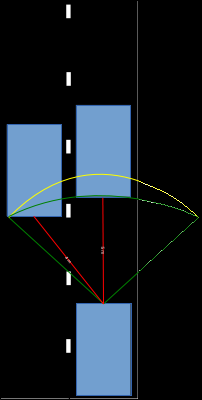
\includegraphics[width=0.3\textwidth]{plaatjes/roadeye-road}
    \caption{Application flow diagram.}
    \label{fig:road-situation}
\end{figure}%

% Conclusies en aanbevelingen moeten verzameld worden in een apart en
% herkenbaar deel van het verslag. Hoewel in het hoofdverslag op diverse
% plaatsen conclusies getrokken kunnen worden, moeten de belangrijkste
% conclusies samengevoegd en samengevat worden. 


% Belangrijk is dat het verschil tussen objectief controleerbare
% conclusies en subjectieve aanbevelingen duidelijk wordt aangegeven.
% Ook is het aan te bevelen om de belangrijkste conclusies conform de
% opdrachtomschrijving te formuleren.

